\documentclass{article}
\usepackage{amssymb}
\usepackage{graphicx}
\usepackage{multicol}
\usepackage{bm}

\usepackage{setspace}
\usepackage[utf8]{inputenc} % allow utf-8 input
\usepackage[T1]{fontenc}    % use 8-bit T1 fonts
\usepackage{hyperref}       % hyperlinks
\usepackage{url}            % simple URL typesetting
\usepackage{booktabs}       % professional-quality tables
\usepackage{amsfonts}       % blackboard math symbols
\usepackage{nicefrac}       % compact symbols for 1/2, etc.
\usepackage{microtype}      % microtypography
\usepackage{lipsum}

\title{Learning with Kernels}
\author{
  Harshita Agarwala\\
  M.Sc in Mathematics in Data Science\\
  Technische Universität München}
  
\begin{document}
\maketitle
\begin{abstract}
This paper describes the central ideas of Support Vector (SV) Classification. Its goal is to provide an overview of the basic concepts. It also gives an introduction to kernels and discusses their use in faster computation of different learning algorithms. It reviews the main kernel algorithms like SV classifiers and Kernel-Principal Component Analysis. It also provides insights from Statistical Learning Theory and presents important mathematical formulations on performance of functions learnt by these algorithms. Moreover, it provides results from a python implementation of the SV classification problem discussed in the paper.
\end{abstract}

\pagebreak
\tableofcontents
\pagebreak



\section{Introduction}
In this context, learning refers to the process of inferring general rules by observing examples. For instance, children can learn what “a car” is, just by being shown examples of objects that are cars and objects that are not cars. The field of machine learning studies the process of learning in the abstract. Machine learning has roots in artificial intelligence, statistics, and computer science, but by now has established itself as a scientific discipline in its own right.

There are two types of learning algorithms: supervised and unsupervised. Classification is an example of a supervised learning problem: the training examples consist both of instances(inputs) and correct labels. Therefore the goal is to find a functional relationship between them. On the other hand, the training data in the unsupervised setting only
consists of instances (inputs), without any further information about what kind of output is expected on those instances. Here, the question of learning is more about learning a structure on the underlying space of instances. A standard example of such a setting is clustering. In this paper, we focus on a classification problem and then go to a form of unsupervised learning.

\section{Data Representation and Similarity}
\label{sec:data_term}
A basic problem of learning theory is assigning a new object to a class given some empirical data or training data.
\begin{equation}
\label{train_data}
  (x_1, y_1), . . . ,(x_m, y_m) \in \chi \times \{\pm 1\}
\end{equation}
Here, $\chi$ is a nonempty set of patterns/inputs $x_i$ and the $y_i$ are called labels, targets, or outputs. This is called (binary) pattern recognition or (binary) classification. To study the problem of learning, an additional kind of structure is required that generalizes to unseen data points. In the case of pattern recognition, this means that given some new pattern $x \in \chi$, the model should be able to predict the corresponding $y \in \{\pm 1\}$.

Intuitively, such a $y$ has to be chosen such that $(x, y)$ is in some sense \textbf{similar} to the training examples in eq  (\ref{train_data}). Hence, notions of similarity in $\chi$ and $\{\pm 1\}$ are needed.

These similarity measures are also referred to as kernels \cite{learn_kernels}. Kernel functions are of the form: \\
$k: \chi \times \chi \rightarrow \mathbb{R}, (a,b) \rightarrow k(a,b)$ 

A simple kernel function is the Dot Product/Scalar Product: $<\textbf{a},\textbf{b}> = \textbf{b}^T\textbf{a}$ where \textbf{a} and \textbf{b} are vectors. The geometric interpretation of the canonical dot product is that it computes the cosine of the angle between the vectors a and b provided they are normalized to unit length: $\cos(\textbf{a},\textbf{b}) = <\textbf{a},\textbf{b}> / (||\textbf{a}|| ||\textbf{b}||)$.

The norm or the length of a vector a is given by: $||\textbf{a}|| = \sqrt{(<\textbf{a},\textbf{a}>)}$. The patterns x can be represented in a dot product space $H$ by a mapping $x \rightarrow \bm{x} = \phi(x)$, here $\bm{x}$ is a vector in the space H (also called Feature Space)

\section{Simple Pattern Recognition Algorithm}
\label{sec:simple_algo}

\begin{figure}
  \centering
  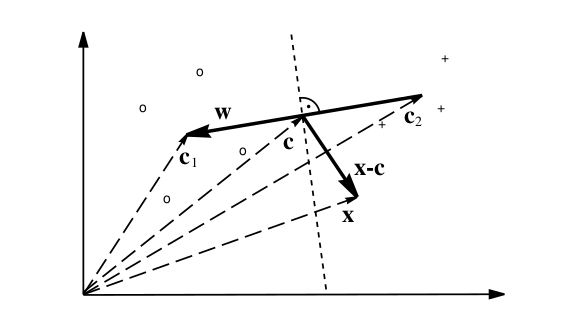
\includegraphics[width=0.7\textwidth]{simple_pattern.png}
  \caption{Simple Pattern Recognition Algorithm}
  \label{fig:fig1}
\end{figure}
We are now in the position to describe a pattern recognition learning algorithm that is one of the simplest possible. We assume that the data is embedded into a dot product space $H$. Using the dot product, we can measure distances in that space. The basic idea of the algorithm will be to assign a previously unseen pattern to the class whose mean is closer.

We first begin by computing the mean of the two classes in feature space $H$:
\begin{equation}
\label{mean1}
    c_1 = \frac{1}{m_1}\sum_{i:y_i = 1}{x_i}
\end{equation}
\begin{equation}
\label{mean2}
    c_2 = \frac{1}{m_2}\sum_{i:y_i = -1}{x_i}
\end{equation}
where $m_1$ and $m_2$ are the number of examples with positive and negative labels,respectively. We assume that $m_1 , m_2 > 0$, that is there exists at least one data point of each label. We then assign a new point $x$ to +1 if it is closer to $c_1$ and -1 if it is closer to $c_2$. From (Figure:\ref{fig:fig1}) we can see the geometric construction can be formulated in terms of the dot product $<. ,.>$. Half-way in between $c_1$ and $c_2$ lies the point $c = (c_1 + c_2 )/2$. We compute the class of x by checking whether the vector $x - c$ connecting $c$ to $x$ encloses an angle smaller than $\pi$/2 with the vector $w = c_1 - c_2$ connecting the class means. This leads to:
\begin{eqnarray}
\label{simple_2}
y & = & sgn <(x-c),w> \nonumber \\
&=& sgn <x-(c_1+c_2)/2,c_1-c_2> \nonumber \\
& = & sgn (<(x,c_1>-<x,c_2> +b)
\end{eqnarray}

where $b$ is defined as $b = \frac{1}{2}(||c_1||^2 + ||c_2||^2)$. It can be clearly seen from (Figure:\ref{fig:fig1}), that the equation (\ref{simple_2}) induces a decision boundary which has the form of a hyperplane.

We first express the equation (\ref{simple_2}) by replacing $c_1$ and $c_2$ with equations (\ref{mean1}) and (\ref{mean2}):
\begin{equation}
    y = sgn(\frac{1}{m_1} \sum_{i:y = 1}{<x,x_i>} + \frac{1}{m_2}\sum_{i:y = -1}{<x,x_i>} + b) \nonumber
\end{equation}
As discussed earlier, the dot products are a kernel. We can then replace them with the function $k: \chi \times \chi \rightarrow \mathbb{R}$,\ $(a,b) \rightarrow k(a,b)$. Hence, the final equations are:
\begin{equation}
    y = sgn(\frac{1}{m_1} \sum_{i:y = 1}{k(x,x_i)} + \frac{1}{m_2}\sum_{i:y = -1}{k(x,x_i)} + b) \nonumber
\end{equation} and then the offset can be written as 
\begin{equation}
    b = \frac{1}{2} (\frac{1}{m_2}^2 \sum_{i:y = -1}{k(x,x_i)} - \frac{1}{m_1}^2 \sum_{i:y = 1}{k(x,x_i)} \ ) \nonumber
\end{equation}

\section{Introduction to Statistical Learning Theory}
 Statistical learning theory (SLT) is a theoretical branch of machine learning and attempts to lay the mathematical foundations for the field. \cite{intro_stat} The questions asked by SLT are fundamental:
\begin{enumerate}
    \item Which learning tasks can be performed by computers in general (positive and negative results)?
\item What kind of assumptions do we have to make such that machine learning can be successful?
\item What are the key properties a learning algorithm needs to satisfy in order to be successful?
\item Which performance guarantees can we give on the results of certain learning algorithms?
\end{enumerate}
Let us first assume that the data is generated independently from some unknown (but
fixed) probability distribution $P(x, y)$. This is usually a standard assumption in learning theory. The data generated this way is called independent and
identically distributed (iid). Hence, now the goal is to find a function $f$ that correctly classifies unseen examples $(x', y')$. In other words $f$ should be a function such $f(x') = y'$ where $(x', y')$ was also generated from the same probability distribution $P(x, y)$.

Accuracy of a function is measured by the zero-loss function $\frac{1}{2} |f(x) - y|$ where loss is 0 on correct classification and 1 on incorrect. We can now define two risk or error functions.
\begin{itemize}
    \item Expectation of True Error: 
    \begin{equation}
        R[f] = \frac{1}{2} \int{|f(x) - y|} \ dP(x,y) \nonumber
    \end{equation}
    This error is the average error over sample points (test points) that were drawn from the underlying distribution P(x,y). This is in general also known as test-error.
    \item Average Empirical Risk: 
    \begin{equation}
        R_{emp}[f] = \frac{1}{2m} \sum_{i=1}^{m}{|f(x_i) - y|}
    \end{equation}
    This error is called the training-error as it is observed only on training data. 
\end{itemize}
As, the underlying distribution is unknown, the main problem in learning theory is to find a function that performs well on the training and test data sets. A function, that minimizes the training data might not minimize the test data. According to Statistical LEarning Theory, a function genaralizes well if $|R[f] - R_{emp}[f]|$ is small. In other words the empirical risk converges to the expectation of true risk. \cite{intro_stat}

\begin{figure}
  \centering
  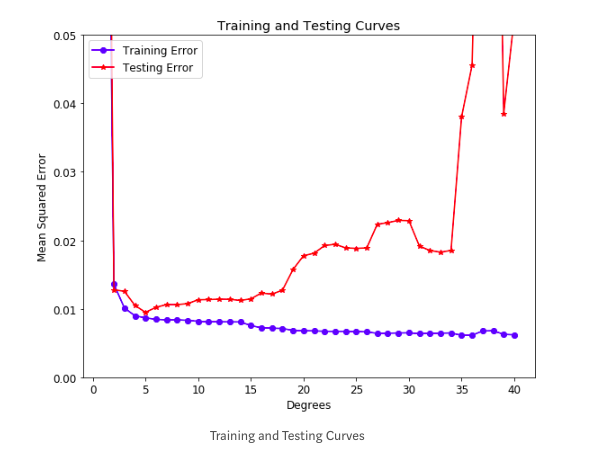
\includegraphics[width=0.8\textwidth]{test-train_error.png}
  \caption{The graph shows how the Testing error increases with more complex models. Here the increase in Degrees imply the increase in degree of a fitted polynomial function $f$.}
  \label{fig:error_fig}
\end{figure}

This issue is commonly referred to as the bias-variance tradeoff. If a simple model is used to find the function $f$ that generalizes well on unseen data then it will have high bias (selection-bias). It might also have high training error. However, if we choose a complicated model that works very well with the training samples, we might have high error on unseen data. This model will then have high variance and low training error. Hence, the tradeoff is to choose a model complex enough to genaralize well on both training and test data points. In (Figure: \ref{fig:error_fig}) we can see how the training error and test error change with increasing complexity.

\subsection{Vapnik–Chervonenkis Theory (VC)}
The VC theory provides a way to restrict the set of functions from which $f$ is chosen, to one which has a capacity(complexity, expressive power, richness, or flexibility) suitable for the amount of training data. There are many capacity measures like the VC dimension, annealed VC entropy or the fat shattering dimension. We will focus on the VC Dimension and hence the VC Bound.

Now, each function of the class, labels the training patterns in a certain way. Since the labels are in \{$\pm$1\}, there are at most $2m$ different combination of labels for $m$ patterns. However, a given class of functions might not be sufficiently rich to induce all these combinations; in other words, it might not be able to shatter the $m$ points. A function with some parameters $\alpha$, is said to \textbf{shatter} $n$ points if for all possible assignments of labels to those points, there exists some $\alpha$ such that the model makes no errors when evaluating that set of data points.  Similarly, for a set of functions, we can say that the set shatters $n$ points when all the functions in the set can shatter at least $n$ points. 

\textbf{VC Dimension} is therefore defined, as the largest $m$ such that there exists a set of $m$ points which the class of functions can shatter, and $\infty$ if no such $m$ exists.

Now, the \textbf{VC Bound} is defined as: Let $h < m$, be the VC dimension of the class of functions that the learning machine can implement, then for all functions of that class, with a probability of at least $1-\sigma$ the following bound holds:
\begin{equation}
\label{VC_dim}
R[f] \leq R_{emp}[f] + \phi \Big(\frac{h}{m} , \frac{\log{\sigma}}{m}\Big)
\end{equation}
here the confidence term (or capacity term) $\phi$ is defined as:
\begin{equation}
\phi \Big(\frac{h}{m} , \frac{\log{\sigma}}{m}\Big) = \sqrt{\frac{h(\log{\frac{2m}{m}+1}) - \log(\sigma/4)}{m}}
\end{equation}
Here also the bias-variance tradeoff can be seen in play. The capacity term $\phi$ is an increasing function of $h$. This means that with increase in $h$, the model will become more complex as it will be able to shatter more points. However, the confidence term increases and therefore the bound on the test error increases. Hence, the training error might drop but as the capacity term $\phi$ increases the bound does not necessarily lessen on the test-error. 

In order to get nontrivial predictions from (\ref{VC_dim}), the function set must be restricted such that its capacity (VC dimension) is small enough (in relation to the available amount of data). At the same time, the class should be large enough to provide functions that are able to model the dependencies hidden in $P(x, y)$. The choice of the set of functions is thus crucial for learning from data.

\section{Support Vector Classification}
Vapnik considered the class of hyperplanes in some dot product
space $H$ to be, $<\bm{w},\bm{x}> + b = 0 \ , \bm{w} \in H, b \in R$ corresponding to the decision function $f(\bm{x}) =  <\bm{w},\bm{x}> + b$. This learning algorithm's assumption is that the class labels are separable by the hyperplane, that is they are linearly separable. Among all the possible hyperplanes there exists a unique optimal hyperplane, distinguished by the maximum margin of separation between any training point and the hyperplane. The optimal hyperplane's form is: \\
\begin{equation*}
    \max_{\bm{w},b} \ \min(||\bm{x} - \bm{x_i}|| : \bm{x} \in H, <\bm{w},\bm{x}> +b =0, i=1,...,m)
\end{equation*}

Moreover, the capacity of the set of possible hyperplanes decreases with increase in margins. Hence, the VC bound improves. Therefore we can say that the optimal hyperplane has a good generalization performance. Additionally, it is computationally attractive, since it can be constructed by solving a quadratic programming problem for which there exist efficient algorithms.

\begin{figure}
  \centering
  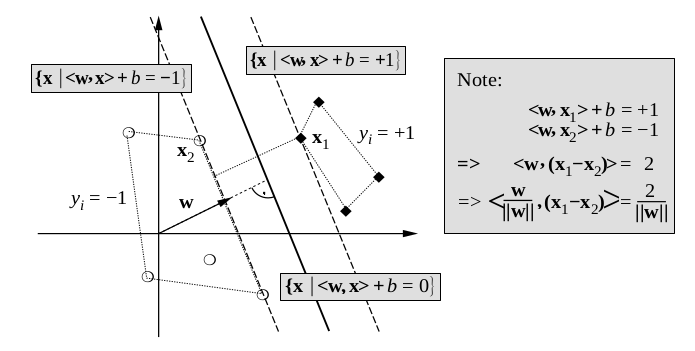
\includegraphics[width=0.8\textwidth]{hyperplane.png}
  \caption{Optimal hyperplane}
    \label{fig:hyperplane}
\end{figure}

The optimal hyperplane in (Figure: \ref{fig:hyperplane}) is shown as a solid line. There exists a weight vector $\bm{w}$ and a threshold $b$ such that 
\begin{equation*}
y_i(<\bm{w}, \bm{x_i} > + b) > 0 \ (i = 1, . . . , m)
\end{equation*} 
. Re-scaling $\bm{w}$ and $b$ such that the point(s) closest to the hyperplane satisfy 
\begin{equation*}
 |<\bm{w}, \bm{x_i}> + b| = 1   
\end{equation*}
, we obtain a canonical form $(\bm{w}, b)$ of the hyperplane, satisfying
\begin{equation*}
 y_i(<\bm{w}, \bm{x_i}> + b) \geq 1   
\end{equation*}
 . In this case, the margin, measured perpendicularly to the hyperplane, equals $2/||\bm{w}||$. This can be seen by considering two points \begin{equation*}
 \textbf{x_1}, \textbf{x_2}
 \end{equation*}
 on opposite sides of the margin, that is, 
 \begin{equation*}
 <\bm{w}, \textbf{x_1}> + b = 1 \ , \ <\bm{w}, \textbf{x_2}> + b = -1
 \end{equation*}
   and projecting them onto the hyperplane
normal vector $\bm{w}/||\bm{w}||$.

Now as we want to maximize the margin which is $2/||\bm{w}||$. We can create a minimizing function of $||\bm{w}||/2$. Therefore, to construct the optimal hyperplane, one has to solve the following constrained optimization problem \cite{kevin,bishop}:
\begin{equation}
\label{eq:primal}
    \min_{\bm{w} \in H, b \in R} f(\bm{w}) = \frac{1}{2}||\bm{w}||^2
\end{equation}
\begin{center}
\begin{equation*}
\textit{subject to } y_i(<\bm{w},\bm{x_i}> + b) \geq1
\end{equation*}
\end{center}
This problem can be solved using Lagrangian Multipliers.

\subsection{Lagrangian and Strong Duality}
Consider the general constrained optimization problem: $\min f(z)$ subject to $c_i(z) \geq 0$ for $ i = 1,...,m$ where $f$ is the main minimization problem and the $c_i$ are constraints on choosing $z$. This is called the primal problem. The corresponding Lagrangian is defined as:
\begin{equation}
\label{eq:lag}
    L(z,\lambda) = f(z) - \sum_{i=1}^M{\lambda_i c_i}
\end{equation}
with Lagrangian multipliers (also called dual variables) $\lambda_i \geq 0$. Based on the Lagrange function we can create a new function that provides a lower bound on the objective function $f$ . Since the dual variables are all positive, i.e. $\lambda_i \geq 0$, we know that $f(z) \geq L(z, \lambda)$ for all feasible $z$. This motivates the definition of the Lagrange dual function as:
\begin{equation}
    g(\lambda) = \inf_{z} L(z,\lambda) = \inf_z \Big( f(z) - \sum_{i=1}^M{\lambda_i c_i} \Big)
\end{equation}
The dual function $g$ is concave, even if the original problem is convex since it is the point-wise infimum of affine functions. The dual form yields lower bounds on the optimal value $p*$ of the objective function $f$ . For any $\lambda \geq 0$ we have $g(\lambda) \leq p^*$. Therefore, the Lagrangian dual problem is to maximize $g$ so that the lower bound on $p^*$ is as close to it as possible. The Lagrangian dual problem is:
\begin{equation}
    \max_\lambda g(\lambda) \ \textit{ s.t } \ \lambda_i \geq 0
\end{equation}
Now we can define strong duality using Slater’s Conditions where the minimum of the primal problem coincides with the maximum of the dual problem, i.e. $d^* = \max_\lambda g(\lambda) =\inf_z f(z) = p^*$
\subsection{Slater's Condition}
Let's again consider the constrained optimization problem in feature space $H$: \\
minimize $f(z)$ subject to $c_i(z) \leq 0$ , $i = 1,2,…,m$. 

Then the Slater's condition \cite{slater} states that:
\begin{itemize}
    \item If $f, c_1,..., c_m$ are convex and there exists an $z \in H$ such that $c_i (z) < 0$, for all $i = 1,2,…,m$
    \item Or $f$ is convex and the constraints are affine, that is
$c_i(z) = w_i^T z + b_i \leq 0$ , for all $i = 1,2,…,m$
\end{itemize}
Then strong duality holds.

Now we can see that in the case of Support Vector Classification, the primal problem is convex and the constraints are all affine. Hence, strong duality holds. Therefore on maximizing the dual problem, we can find the minimum of the primal problem.

\subsection{Karush-Kuhn-Tucker Conditions (KKT Conditions)}
These conditions on Lagrangian multipliers along with strong duality are used to further solve. If we have the following optimization problem minimize $f(z)$ subject to $c_i(z) \geq 0 , i = 1,..., m$
with $f , c_1,..., c_m$ convex and strong duality holds, then the following statement is true:

$z^*$ and $\lambda^*$ are the optimal solutions of the constrained optimization problem and the corresponding Lagrange dual problem if and only if they satisfy the Karush-Kuhn-Tucker (KKT) conditions:
\begin{eqnarray}
c_i(z^*) \geq 0 & \textit{primal feasibility},\\
\lambda_i^* \geq 0 & \textit{dual feasibility},\\
\lambda_i^* c_i(z^*) = 0 & \textit{complementary slackness},\\
\triangledown_z L(z^*, \lambda^* ) = 0 & z^* \textit{minimizes Lagrangian}
\end{eqnarray}
\begin{center}
    for all $i = 1,..., m$
\end{center}
\subsection{Solving Support Vector Classification Algorithm}
The Lagrangian of this model will be given by combining equations \ref{eq:primal} and \ref{eq:lag}:
\begin{center}
\begin{equation*}
    L(\bm{w},b,\bm{\lambda}) = \frac{1}{2} ||\bm{w}||^2 - \sum_{i=1}^{m}{\lambda_i(y_i(<\bm{x_i},\bm{w}> +b) -1)}
\end{equation*}
\end{center}
here $\bm{\lambda} = (\lambda_1,...,\lambda_m)$. Now the derivatives of L w.r.t $\bm{w}$ and $b$ is:
\begin{equation*}
    \triangledown_w L = w + \sum_{i=1}^{m}{\lambda_iy_i\bm{x_i}}
\end{equation*} and 
\begin{equation*}
    \triangledown_b L = \sum_{i=1}^{m}{\lambda_iy_i}
\end{equation*}
As strong duality holds and the primal and constraints are all convex functions, we can use KKT conditions to further solve this problem. Now we can equate the derivative of Lagrangian to 0 (19). This gives us:
\begin{eqnarray}
\bm{w} = \sum_{i=1}^{m}{\lambda_iy_i\bm{x_i}} & \sum_{i=1}^{m}{\lambda_iy_i} =0
\end{eqnarray}
This further leads to the dual problem of
\begin{eqnarray}
    \max_{\bm{\lambda}} g(\bm{\lambda}) & = & \frac{1}{2} \sum_{i,j=1}^{m}{\lambda_i\lamda_jy_iy_j\bm{x_i}\bm{x_j}} -  \sum_{i,j=1}^{m}{\lambda_i\lamda_jy_iy_j\bm{x_i}\bm{x_j}} - b\sum_{i=1}^m{\lambda_iy_i} + \sum_{i=1}^m{\lambda_i} \nonumber \\
    & = & \sum_{i=1}^m{\lambda_i} - \frac{1}{2} \sum_{i,j=1}^{m}{\lambda_i\lamda_jy_iy_j\bm{x_i}\bm{x_j}}
\end{eqnarray}
subject to $\lambda_i \geq 0, \ i = 1,...,m$ and $\sum_{i=1}^{m}{\lambda_iy_i} =0$. This is solved using a Quadratic program (QP) solver for $\bm{\lambda}$ through which $\bm{w}$ and $b$ can also be solved. The final discussion is of the form:
\begin{equation}
    f(\bm{x}) = sgn \Big( \sum_{i=1}^{m}{y_i\lambda_i^*\bm{xx_i}} + b^* \big)
\end{equation}
Here $b^*$ and $\lambda_i^*s$ are the optimal values of $b$ and $\lambda_is$.

Combining equation (20) and the complementary slackness condition under KKT:\\
For $\lambda_i$ non-zero we have \begin{equation*}
    y_i(<\bm{x_i} , \bm{w}> + b) -1 = 0
\end{equation*}. This implies that for $\lambda_i$ non-zero the $\bm{x_i}$ lies on one of the margins. These are the points that contribute to the value of $\bm{w}$ and play a role in the optimization. As for all other $\lambda_i = 0$, $\bm{w}$ does not change. These data points are called \textbf{support vectors}.


\begin{figure}
  \centering
  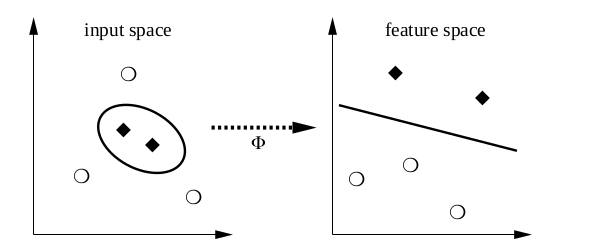
\includegraphics[width=0.7\textwidth]{kernel.png}
  \caption{Kernel on Input Space}
  \label{fig:fig4}
\end{figure}

\subsection{Kernel Trick}
If the input space is not linearly separable (Figure \ref{fig:fig4}) then a mapping $\phi$ can be used to map the training data into a higher-dimensional feature space where the points are linearly separable. This yields a nonlinear decision boundary in input space. By the use of a kernel function, it is possible to compute the separating hyperplane without explicitly carrying out the mapping into the high-dimensional feature space. This is referred to as the kernel trick.
Now we have a dot product in our earlier decision function (22) $<\bm{x},\bm{x_i}>$ which can be written as:
\begin{equation}
<\bm{x},\bm{x_i}> = <\phi(x),\phi(x_i)> = k(x,x_i)
\end{equation}
The kernel trick can be applied since all feature vectors only occurred in dot products. The weight vector then becomes an expansion in feature space, and therefore will typically no longer correspond to the $\phi$-image of a single vector from input space. We thus obtain decision functions of the form:
\begin{equation}
    f(\bm{x}) = sgn \Big( \sum_{i=1}^{m}{y_i\lambda_i^*k(x,x_i)} + b^* \big)
\end{equation} which is obtained through solving the quadractic problem:
\begin{equation}
\max_{\bm{\lambda}} g(\bm{\lambda}) = \sum_{i=1}^m{\lambda_i} - \frac{1}{2} \sum_{i,j=1}^{m}{\lambda_i\lamda_jy_iy_jk(x_i,x_j)}
\end{equation}subject to $\lambda_i \geq 0, \ i = 1,...,m$ and $\sum_{i=1}^{m}{\lambda_iy_i} =0$.

\section{Kernel PCA}
Standard PCA reduces the dimensionality of the observed data by projecting it onto a linear subspace. The projection is chosen in a way that the error measured in the squared standard Euclidean norm is minimized.

Let $\bm{X} \in \bm{R}^{p * n}$ be the centered data matrix and let $\bm{K} := \bm{X^T X}$ be the (n × n)-matrix consisting of all inner products of the data. This is called the Gram Matrix. More precisely, the $(i, j)$ entry of $\bm{K}$ is the inner product $\bm{x_i^T x_j}$ of the i-th and the j-th input points.

Let $\bm{X} = \bm{U \Sigma V^T}$ be the SVD of the data matrix, then the first k principle components of a data vector $\bm{y} \in \bm{R}^p$ are given by $\bm{U_k^T y}$. Here the eigen-value decomposition of $\bm{K}$ helps. Replacing the value of $\bm{X}$ in $\bm{K}$, we get: 
\begin{equation}
\label{kpca}
\bm{K} = \bm{V \Sigma^T \Sigma V^T}    
\end{equation}

Here, $\bm{V}$ is orthonormal and $\bm{\Sigma^T \Sigma}$ is the diagonal. Thus, Equation (\ref{kpca}) is the eigenvalue decomposition of $\bm{K}$, due to the uniqueness of the Eigen Value Decomposition, and by computing the k largest eigenvalues of $\bm{K}$ with their respective eigenvectors, we obtain $\sigma_1^2 ,..., \sigma_k^2$ and $\bm{V_k}$. We can now also write $\bm{\Sigma_k}$ as $diag(\sigma_1 ,..., \sigma_k).$

Now to compute $\bm{U_k^T y}$ we first have:
\begin{eqnarray*}
    \bm{V_k^T X^T y} & = & \bm{V_k^T V \Sigma U^T y}\\
    & = & [ I_k | 0] \bm{\Sigma U^T y}\\
    & = & [ \bm{\Sigma_k} | 0] \bm{U^T y}\\
        & = & \bm{\Sigma_k} \bm{U^T y}\\
\end{eqnarray*}
By multiplying this equation with $\bm{\Sigma_k^{−1}}$ , we obtain: 
\begin{eqnarray}
\label{kpca2}
    \bm{U^T y} &=& \bm{\Sigma_k^{−1}} \bm{V_k^T X^T y} \nonumber \\  &=&\bm{\Sigma_k^{−1}} \bm{V_k^T} [\bm{x_1^T y},..., \bm{x_n^T y}]^{\bm{T}}
\end{eqnarray}
Now we can see that for a new measurement $\bm{y}$, the first k principal components is given by eq (\ref{kpca2}) which can now be computed only through inner products of the data, namely the Gram Matrix $\bm{K}$ and the inner products of $\bm{x_i^T y}$. This can also be extended for a general kernel function by replacing the inner product $\bm{x^Ty}$ by $<\phi(\bm{x}), \phi(\bm{y})> = k(\bm{x},\bm{y})$
\section{Common Kernel Functions}
Some common kernel functions used are:
\begin{itemize}
    \item Polynomial Kernel:
    \begin{equation*}
        k(x, x’) = <x, x’>^d, 
    \end{equation*} where d denotes the degree.
    \item Gaussian or Radial Basis Kernel: 
    \begin{equation*}
        k(x, x') = \exp\Big( \frac{- ||x - x'||2}{2\sigma^2}\Big)
    \end{equation*} (In Python the formula used for RBF kernel is $\exp(- \sigma||x - x’||^2)$    
\item Sigmoid Kernel: $k(x, x’) = \tanh(\gamma <x,x’> + \phi)$
\end{itemize}
By the use of kernels, the optimal margin classifier was turned into a high-performance classifier. Surprisingly, it was noticed that the polynomial kernel, gaussian and sigmoid kernel with suitable choices of $d \in \bm{N}$ and $\sigma, \gamma, \phi \in \bm{R}$ empirically led to SV classifiers with very similar accuracies. In this sense, the SV set seems to characterize (or compress) the given task in a manner which to some extent is independent of the type of kernel (that is, the type of classifier) used.
\section{Results from Python Implementation}

\begin{figure}[h!]
  \centering
  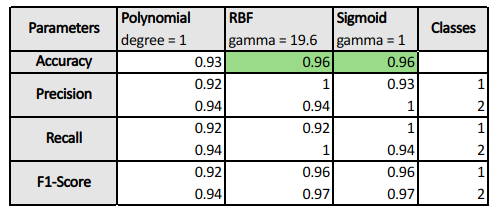
\includegraphics[width=0.6\textwidth]{2class_table.png}
  \caption{Results from Support Vector Classification for 2 classes}
  \label{fig:fig5}
\end{figure}

\begin{figure}[h!]
  \centering
  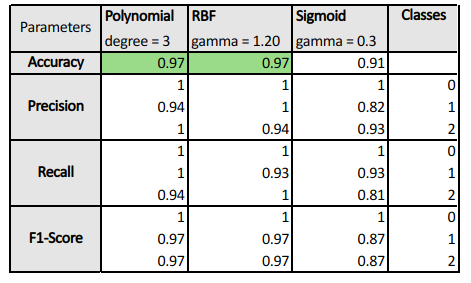
\includegraphics[width=0.6\textwidth]{3class_table.png}
  \caption{Results from Support Vector Classification for 3 classes}
  \label{fig:fig6}
\end{figure}
From the summaries in figures 5 and 6, it can be clearly seen that with the right choice of the parameters, once can get a same level of performance from different kernels. Hence, Support Vector Classification algorithm in itself is a very strong tool.
\\
Decision boundaries results for 2 class and 3 class SV classifier with best performing kernels:
\begin{figure}
  \centering
  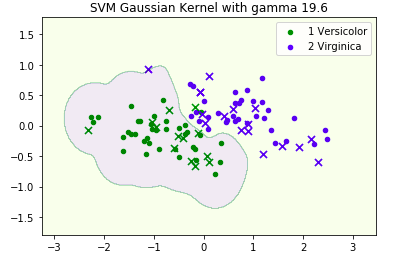
\includegraphics[width=0.6\textwidth]{2class_rbf.png}
  \caption{Decision Boundary for RBF kernel for 2 classes}
  \label{fig:fig7}
\end{figure}
\begin{figure}
  \centering
  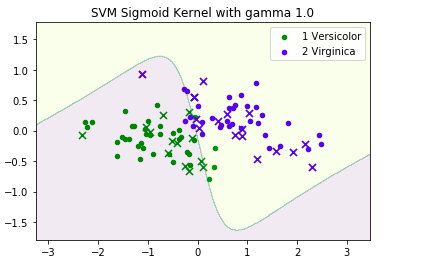
\includegraphics[width=0.65\textwidth]{2class_sigmoid.png}
  \caption{Decision Boundary for Sigmoid kernel for 2 classes}
  \label{fig:fig8}
\end{figure}
\begin{figure}
  \centering
  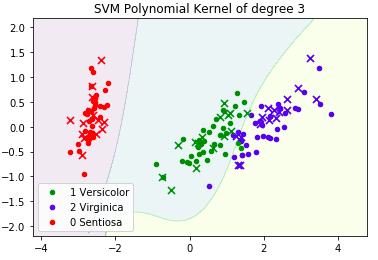
\includegraphics[width=0.6\textwidth]{3class_poly.png}
  \caption{Decision Boundary for Polynomial kernel for 3 classes}
  \label{fig:fig9}
  \end{figure}
\begin{figure}
  \centering
  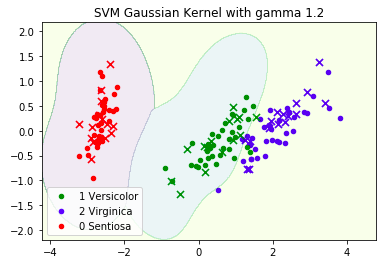
\includegraphics[width=0.6\textwidth]{3class_rbf.png}
  \caption{Decision Boundary for RBF kernel for 3 classes}
  \label{fig:fig9}
  \end{figure}

\section{Summary}
SV classifiers have proved to be a strong classification algorithm because of easy computations and mappings to feature space through kernels. Moreover, many Quadractic Solvers are readily available to solve the dual problem. The RBF kernel in general performs well, as we saw from Section 8. SV classifier has fewer parameters to train or tune. Hence, they are faster. Most importantly, it is a convex problem and therefore guarantees a global optimum.
  
\pagebreak
\bibliographystyle{unsrt}  


\begin{thebibliography}{1}

\bibitem{learn_kernels}
Bernhard Schölkopf and Alexander J. Smola, \textit{"Learning with Kernels"}
\newblock In \url{https://www.cs.utah.edu/~piyush/teaching/learning-with-kernels.pdf}, pages 1--22, Massachusetts Institute of Technology, 2000.

\bibitem{intro_stat}
Ulrike von Luxburg and Bernhard Schölkopf,\textit{"Statistical Learning Theory: Models, Concepts, and Results"}
\newblock In \url{http://www.tml.cs.uni-tuebingen.de/team/luxburg/publications/StatisticalLearningTheory.pdf}, 2008.

\bibitem{bishop}
Christopher M. Bishop, \textit{"Pattern Recognition and Machine Learning"}
\newblock "Springer", pages 291--353, 2006.

\bibitem{kevin}
Kevin P. Murphy, \textit{"Machine Learning: A Probabilistic Perspective"}
\newblock "The MIT Press", pages 475--512, 2012 

\bibitem{slater}
Stephen Boyd and Lieven Vandenberghe,\textit{"Convex Optimization"}
\newblock In \url{https://web.stanford.edu/~boyd/cvxbook/bv_cvxbook.pdf}, pages 215 -- 250, Cambridge University Press, 2004.

\end{thebibliography}


\end{document}
